%!TEX encoding = UTF-8 Unicode

%!TEX root = ../compendium.tex

\Lab{\LabWeekFIVE}

\begin{Goals}
\item Kunna använda vektorer.
\item Kunna använda SHUFFLE-algoritmen för blandning
\item Kunna räkna frekvenser.
\end{Goals}

\begin{Preparations}
\item Läs igenom så att du förstår SHUFFLE-algoritmen.
\end{Preparations}

\subsection{Bakgrund}

Denna labb handlar om kortblandning. Att blanda kort så att varje möjlig permutation (ordning som korten ligger i) är lika sannolik är icke-trivialt; en osystematiskt blandning leder till en skev fördelning. Givet en bra slumpgenerator går det att blanda en kortlek genom att lägga alla kort i en hög och sedan ta ett slumpvist kort från högen och lägga det överst i leken, tills alla kort ligger i leken. Fisher-Yates-algoritmen, som ibland även kallas för en Knuth-shuffle, fungerar på det sättet. I detta kompendium kommer den att benämnas SHUFFLE.

\begin{algorithm}[H]
 \SetKwInOut{Input}{Indata}
 \Input{Array $xs$ som ska blandas}
 $len \leftarrow$ antalet element i $xs$ \\
 \For{$i \leftarrow (len - 1)$ \KwTo $0$}{
  $r \leftarrow$ slumptal mellan $0$ och $i$ \\
  $temp \leftarrow xs(i)$ \\
  $xs(i) \leftarrow xs(r)$ \\
  $xs(r) \leftarrow temp$ \\
 }
\end{algorithm}

Kortspelet poker handlar om att dra kort och få upp vissa kombinationer av kort, s.k. ``händer''. Dessa är ordnade från bättre till sämre; den spelare vinner som fått bäst hand.
Det är därför intressant att veta med vilken sannolikhet en viss hand dyker upp vid dragning från en blandad kortlek.

De vanliga pokerhänderna är, i fallande värde, färgstege (straight flush), fyrtal, kåk (full house), färg (flush), stege (straight), triss, tvåpar och par. Dessa finns illustrerade i labbhandledningen.
Ofta finns ytterligare en hand, s.k. ``royal flush'', men dess sannolikhet är för låg för att kunna simuleras fram på rimlig tid.

\subsection{Obligatoriska uppgifter}

\Task 

\Subtask Implementera metoden \code{shuffle} i klassen \code{CardDeck}. Följ algoritmen noga, och använd \code{cards.length} för att få fram längden på kortleken. 

\Subtask Kör \code{TestingDeck} för att testa att blandningen är jämnt fördelad. \code{TestingDeck} blandar en kortlek med tre kort och räknar hur ofta olika permutationer dyker upp. Du bör få en utskrift med sex ($3!$) ungefär lika långa staplar.

\Task Fyll i de ofärdiga delarna av klassen \code{CardDeck}.

\Subtask Skriv kod för att skapa en array innehållande en 52-korts standardlek. Använd konstanterna i \code{Card}. Tänk på att en \code{for}/\code{yield}-sats inte nödvändigtvis ger en \code{Array}, men att alla samlingar kan omvandlas till en sådan med \code{toArray}.

\Subtask Kör \code{CardDeck} och kontrollera så att du får kort av alla fyra färger, och både ess och kungar.

\Task Använd den färdiga \code{CardDeck}-klassen för att ta fram sannolikheterna för att  ``straight flush'', ``straight'' eller ``flush'' dyker upp.

\Subtask Implementera funktionen \code{test} i \code{PokerProbability}. Använd de färdiga funktionerna \code{Hand.drawFrom} och \code{testHand} för att dra och klassificera en hand från en kortlek. Lagra frekvenserna i en muterbar \code{Map} (\code{collection.mutable.Map} finns redan importerad).

\Subtask Kör \code{PokerProbability}, förslagsvis med 1000 000 iterationer. Du bör få ungefär \\
\begin{tabular}{ll}
Straight flush & 0.00154\%  \\
Flush          & 0.197\%    \\
Straight       & 0.39\%     \\
High card      & 99.41\%
\end{tabular}

% Bilder på respektive korthand med förklarande bildtext för dem som inte vet?

\begin{figure}[h]
 \begin{minipage}[c]{0.5\textwidth}
  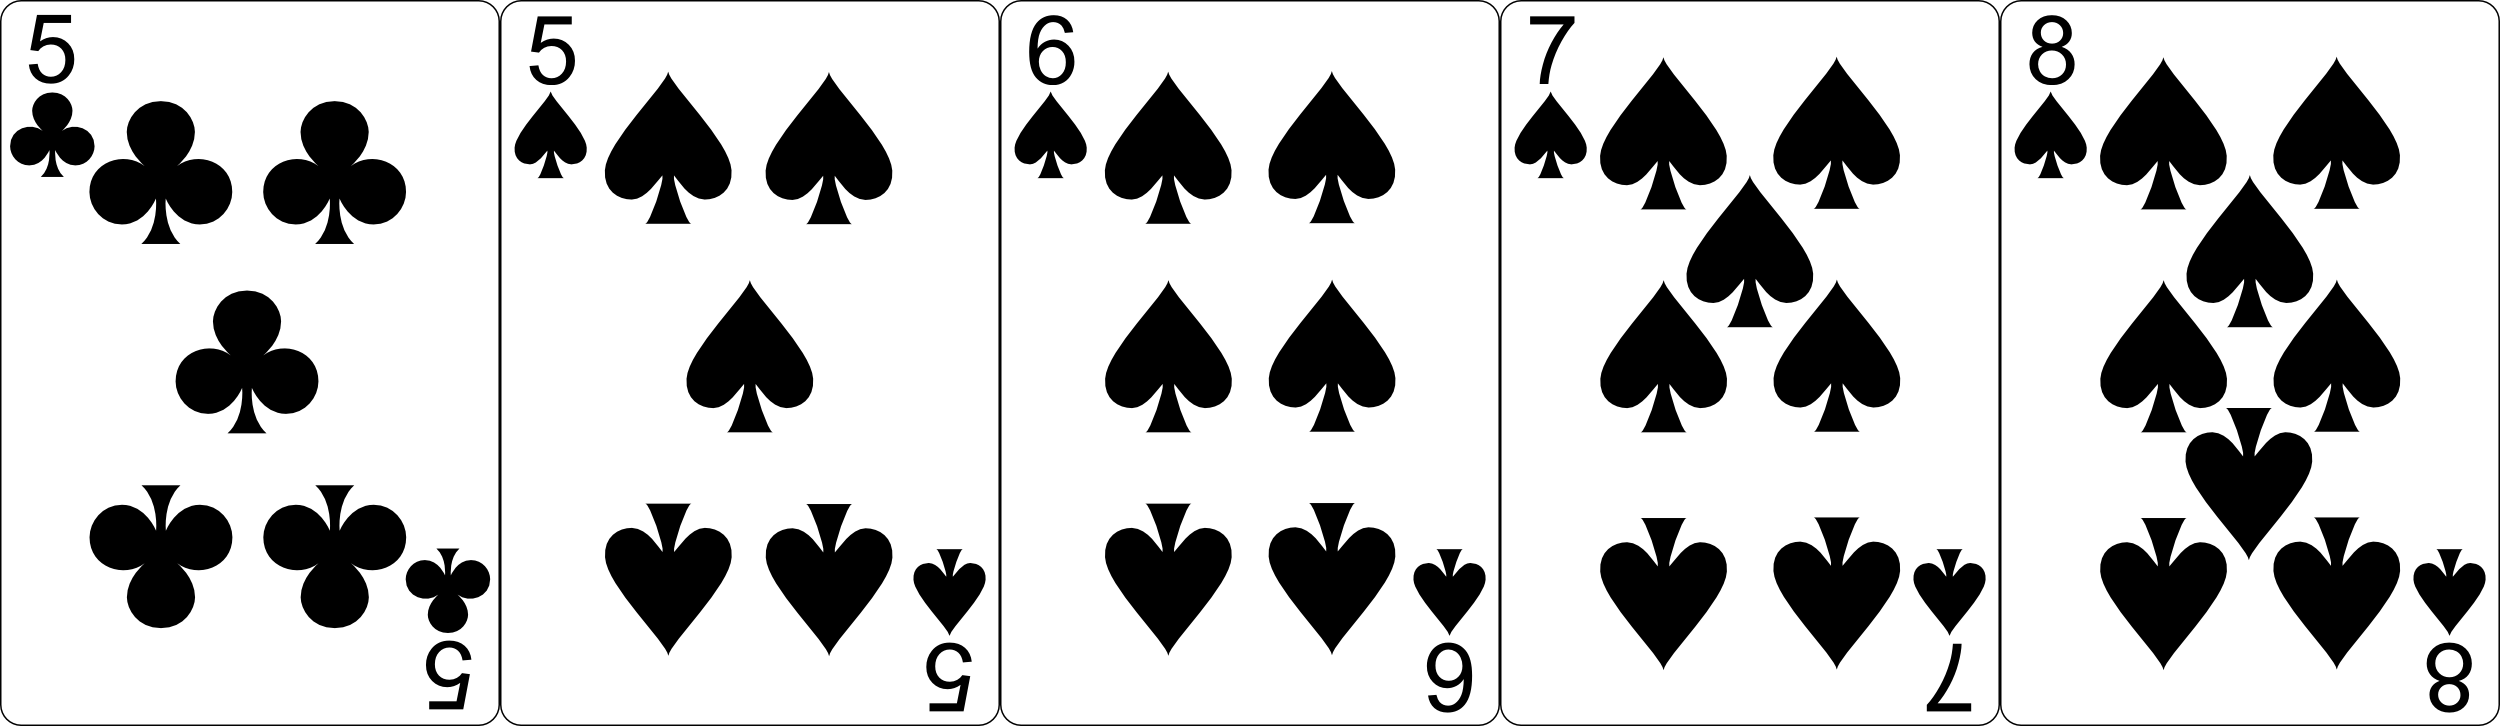
\includegraphics[width=\textwidth]{../img/w05-hands/pair.png}
 \end{minipage}
 \begin{minipage}[c]{0.3\textwidth}
  \caption{Par - två kort har samma valör}
 \end{minipage}
\end{figure}

\begin{figure}[h]
 \begin{minipage}[c]{0.5\textwidth}
  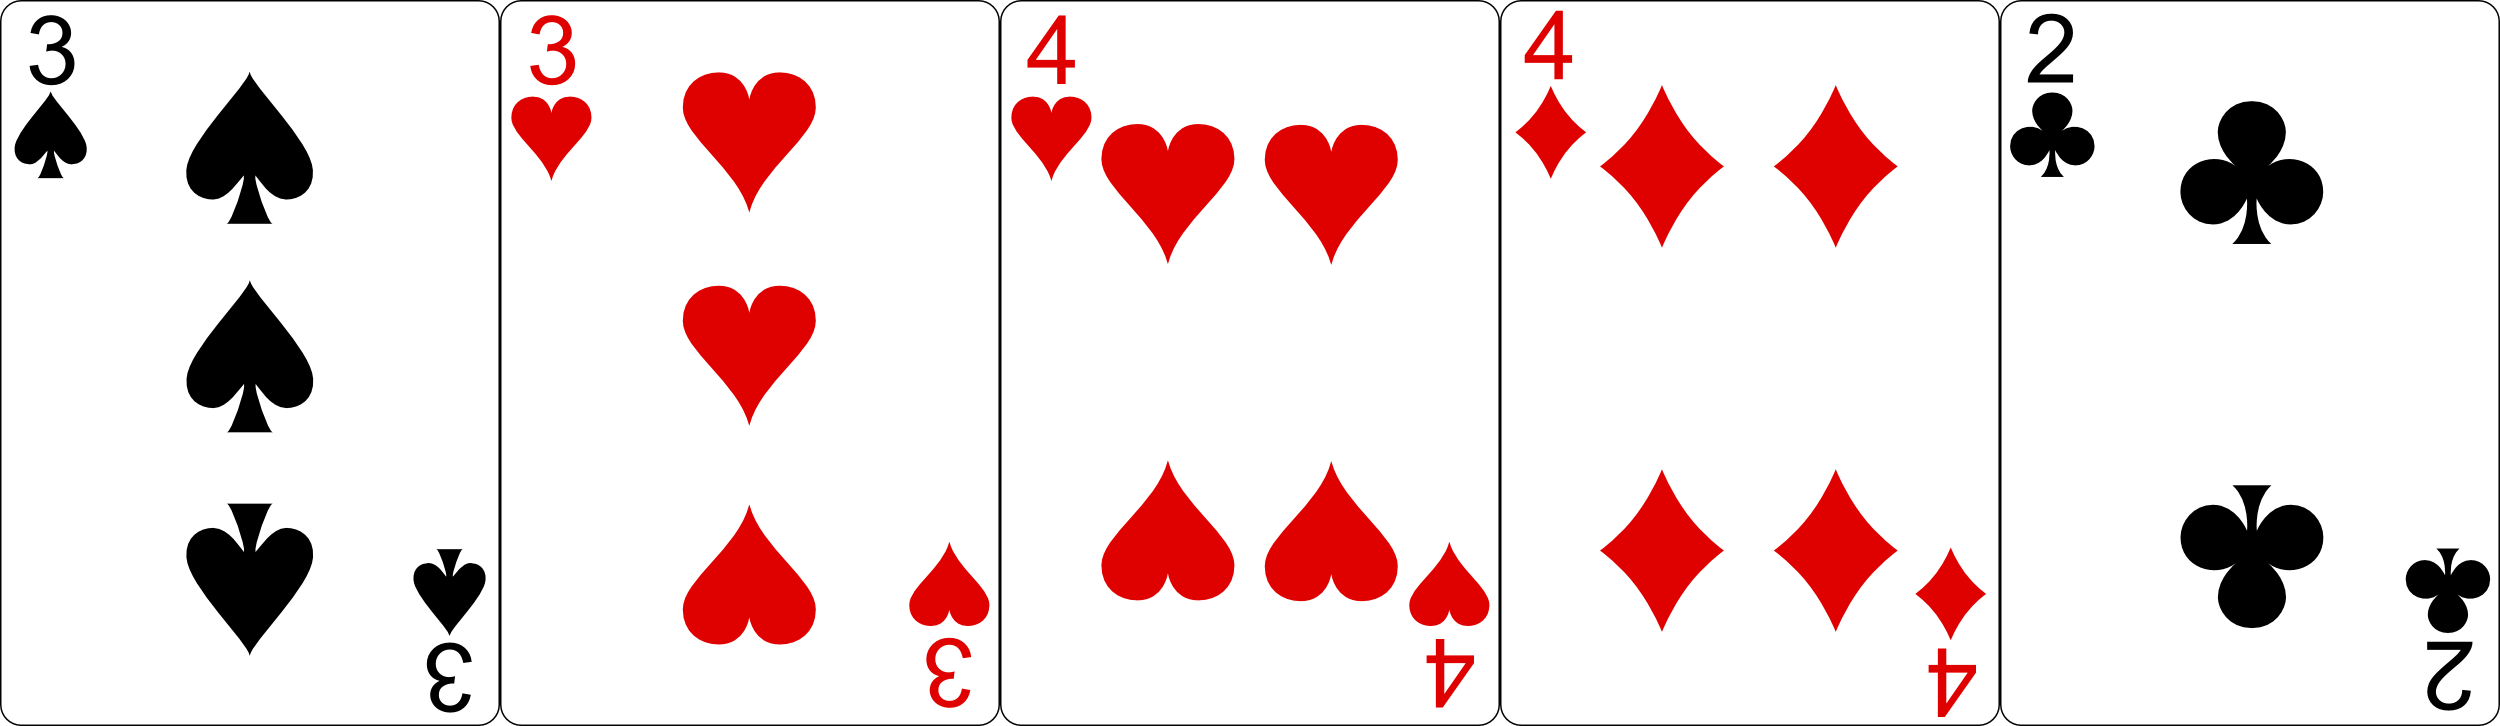
\includegraphics[width=\textwidth]{../img/w05-hands/twopair.png}
 \end{minipage}
 \begin{minipage}[c]{0.3\textwidth}
  \caption{Tvåpar - två olika par}
 \end{minipage}
\end{figure}

\begin{figure}[h]
 \begin{minipage}[c]{0.5\textwidth}
  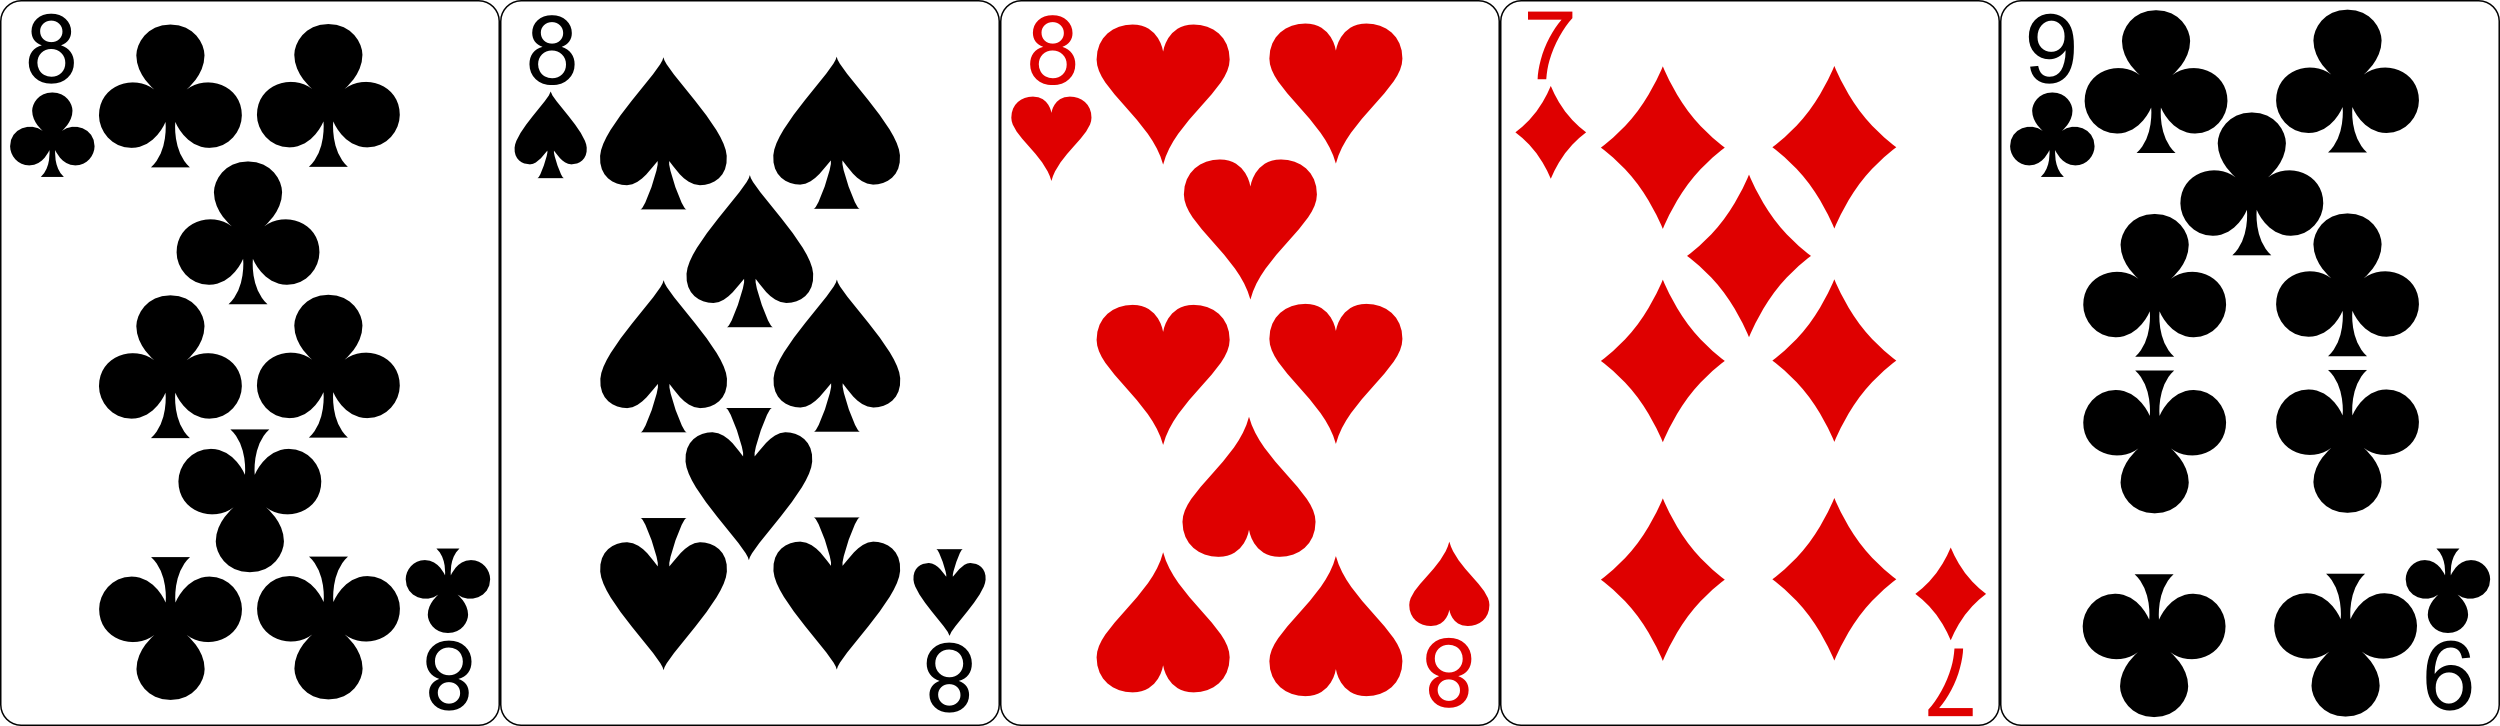
\includegraphics[width=\textwidth]{../img/w05-hands/trips.png}
 \end{minipage}
 \begin{minipage}[c]{0.3\textwidth}
  \caption{Triss - tre kort har samma valör}
 \end{minipage}
\end{figure}

\begin{figure}[h]
 \begin{minipage}[c]{0.5\textwidth}
  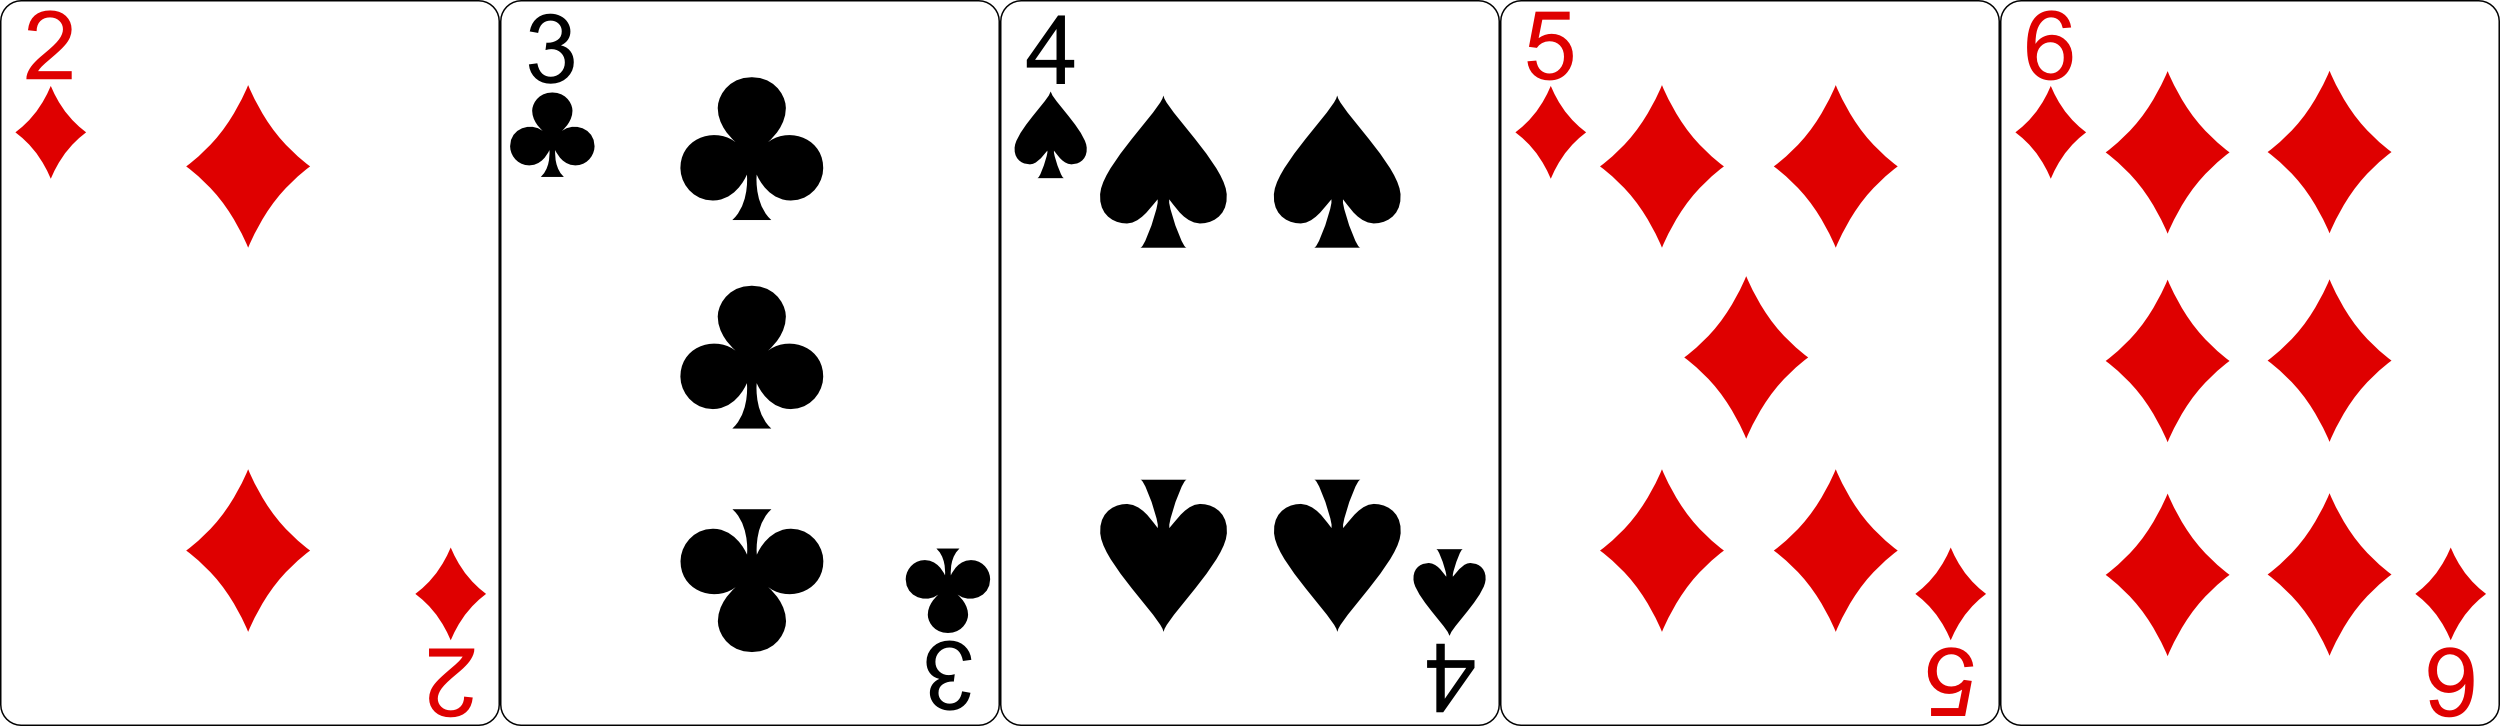
\includegraphics[width=\textwidth]{../img/w05-hands/straight.png}
 \end{minipage}
 \begin{minipage}[c]{0.3\textwidth}
  \caption{Stege - kortens valörer bildar en följd, ess kan vara antingen 1 eller 14}
 \end{minipage}
\end{figure}

\begin{figure}[h]
 \begin{minipage}[c]{0.5\textwidth}
  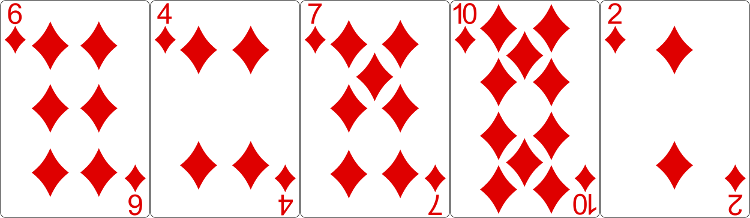
\includegraphics[width=\textwidth]{../img/w05-hands/flush.png}
 \end{minipage}
 \begin{minipage}[c]{0.3\textwidth}
  \caption{Färg - alla kort har samma färg}
 \end{minipage}
\end{figure}

\begin{figure}[h]
 \begin{minipage}[c]{0.5\textwidth}
  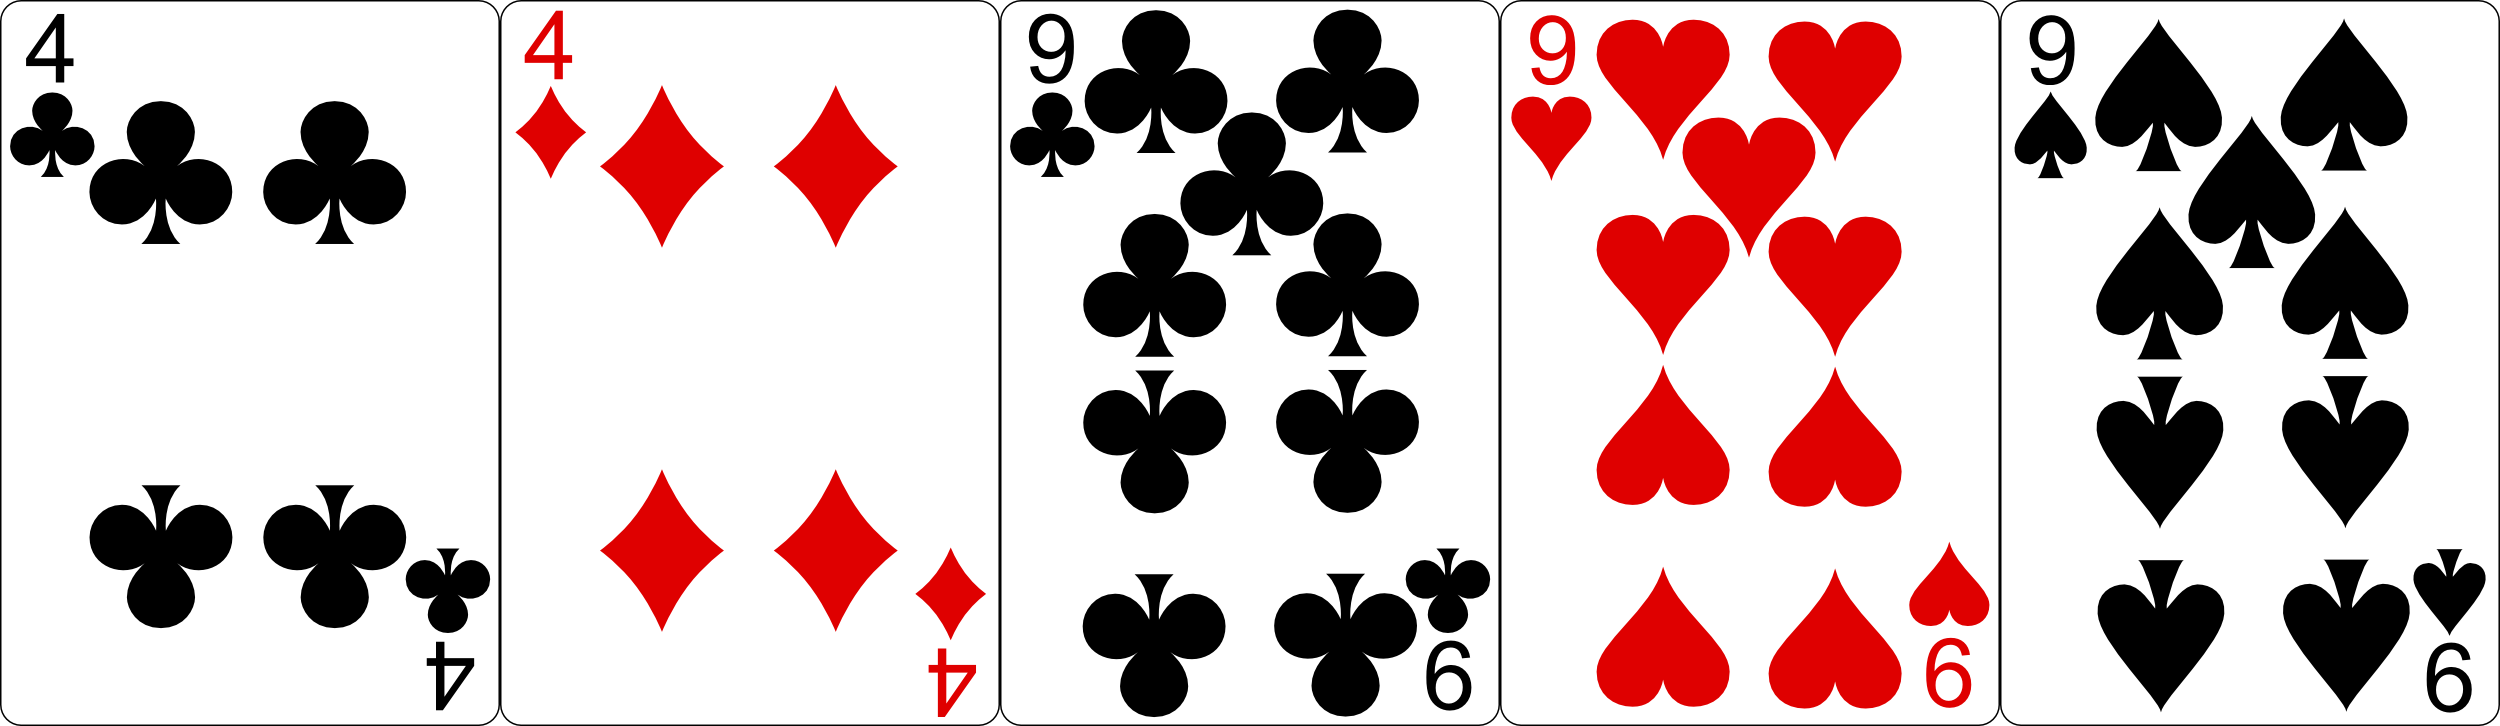
\includegraphics[width=\textwidth]{../img/w05-hands/fullhouse.png}
 \end{minipage}
 \begin{minipage}[c]{0.3\textwidth}
  \caption{Kåk - både triss och par}
 \end{minipage}
\end{figure}

\begin{figure}[h]
 \begin{minipage}[c]{0.5\textwidth}
  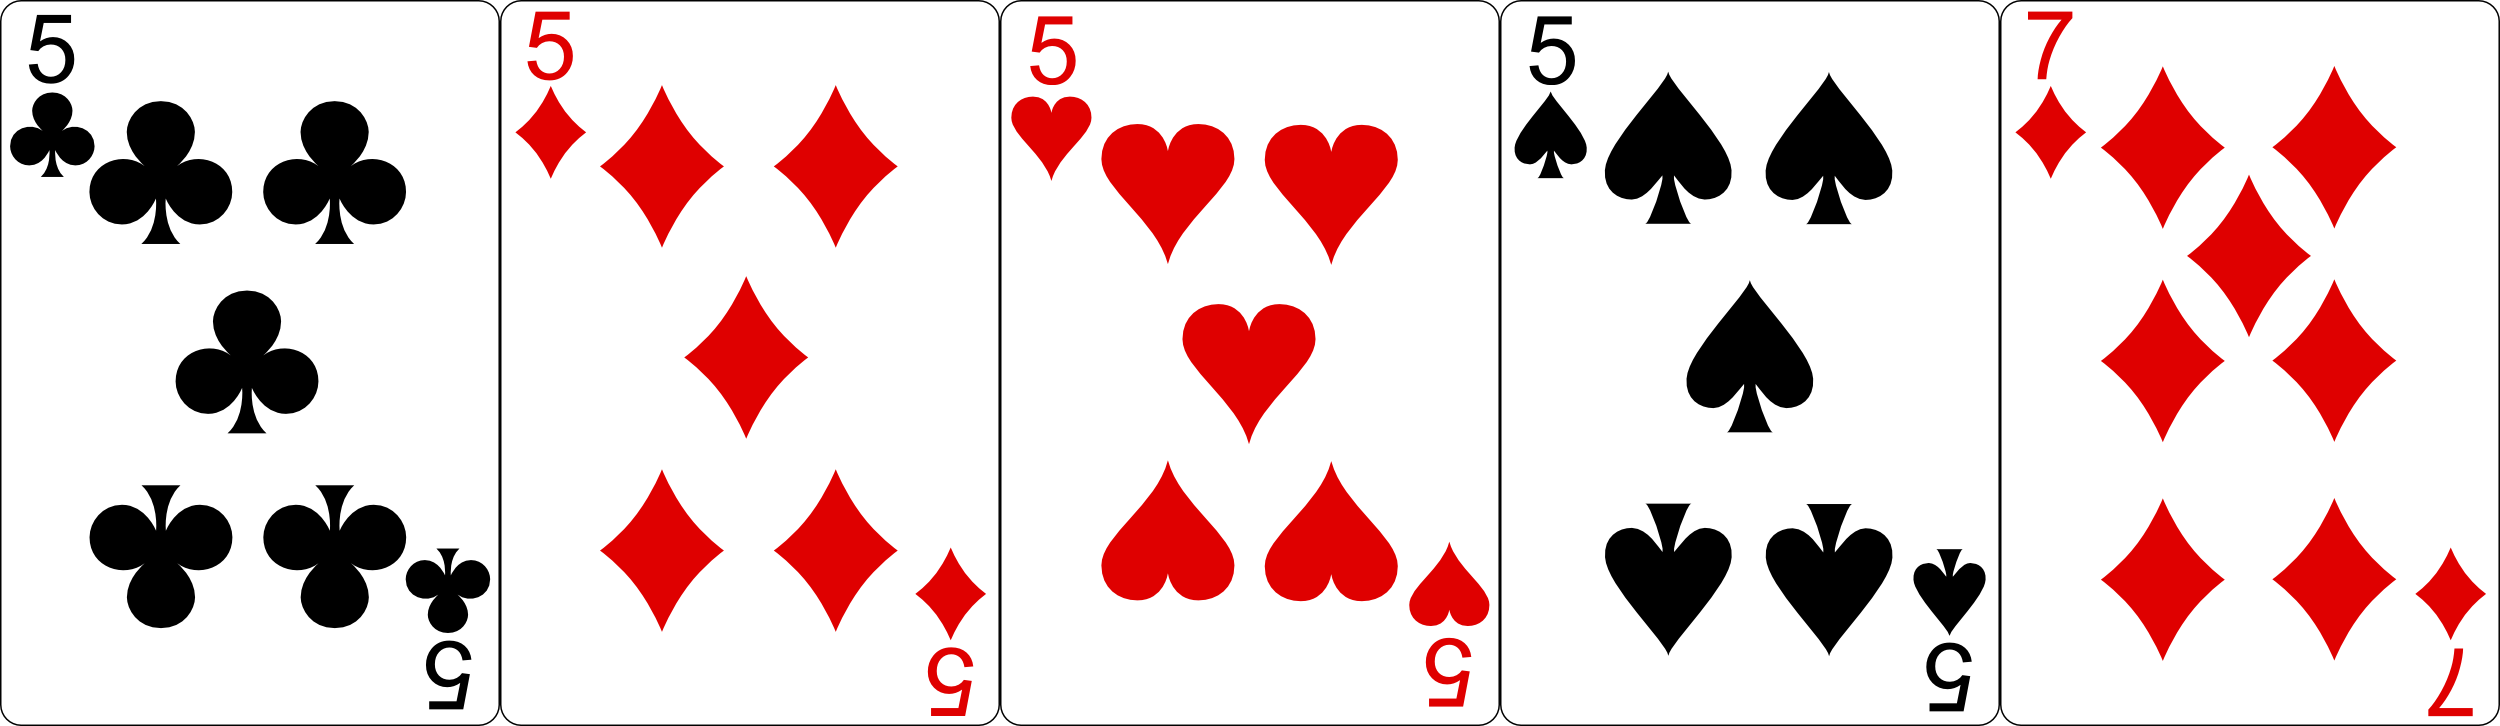
\includegraphics[width=\textwidth]{../img/w05-hands/fours.png}
 \end{minipage}
 \begin{minipage}[c]{0.3\textwidth}
  \caption{Fyrtal - fyra kort har samma valör}
 \end{minipage}
\end{figure}

\begin{figure}[h]
 \begin{minipage}[c]{0.5\textwidth}
  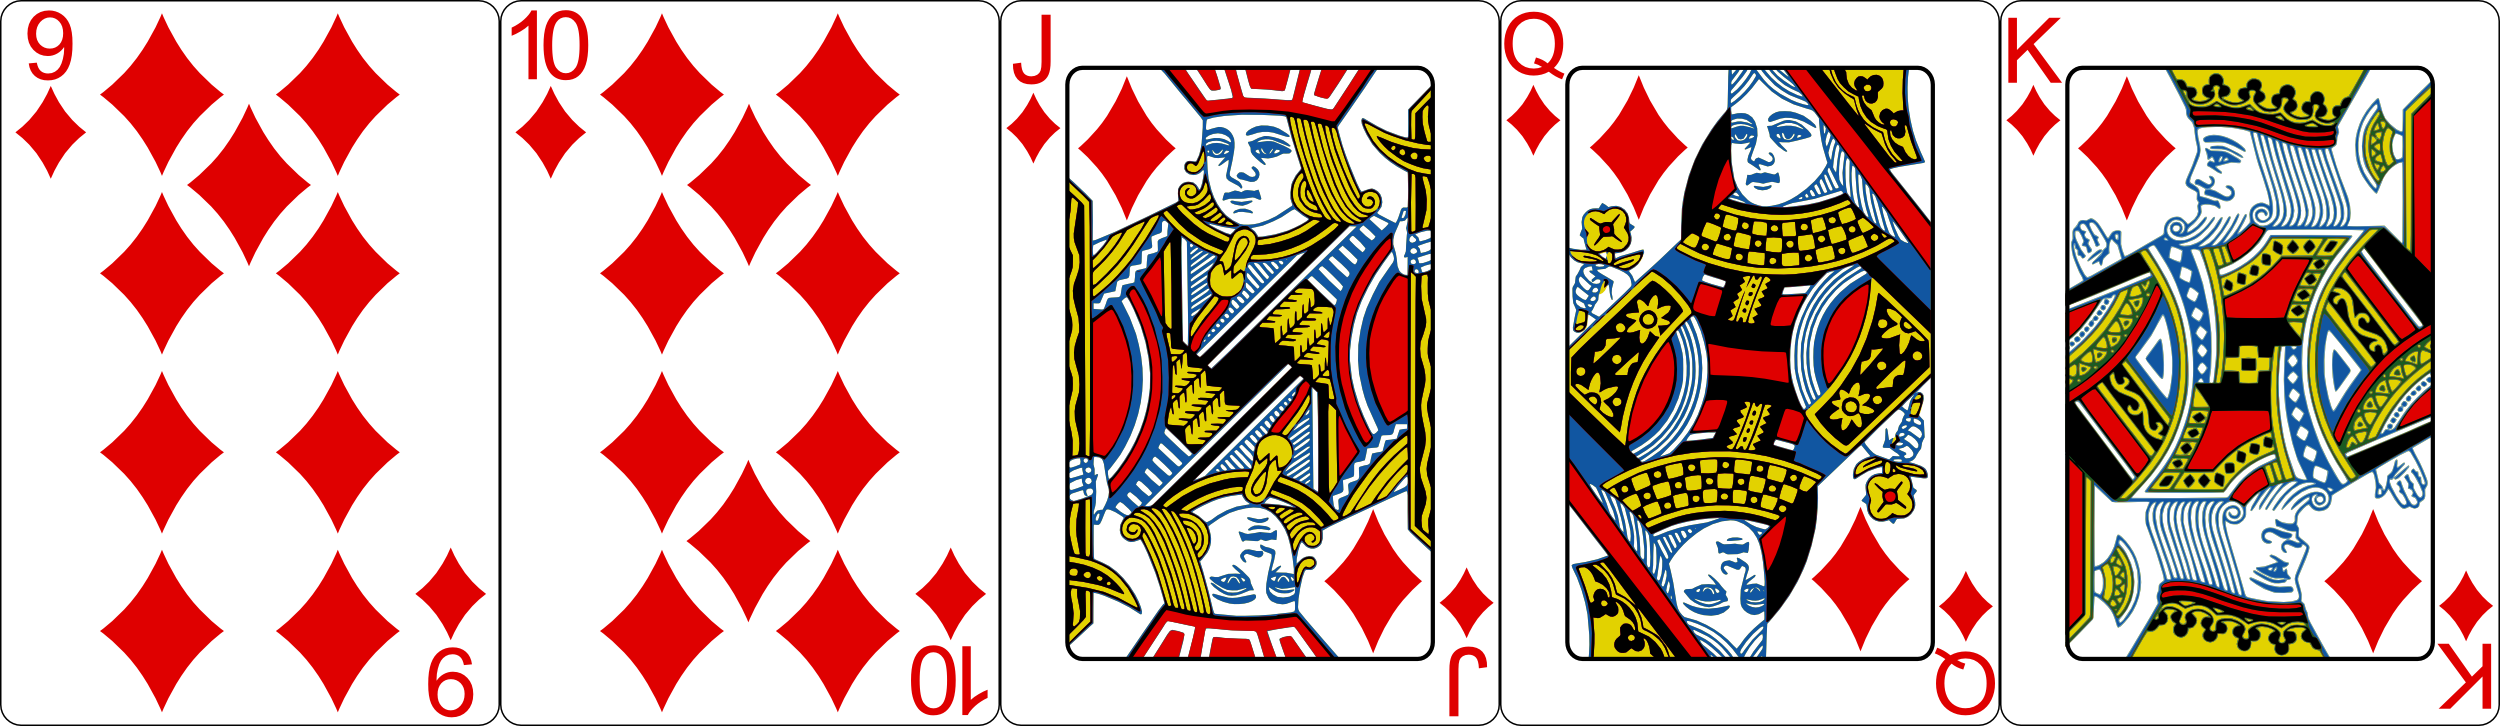
\includegraphics[width=\textwidth]{../img/w05-hands/straightflush.png}
 \end{minipage}
 \begin{minipage}[c]{0.3\textwidth}
  \caption{Färgstege - både stege och färg}
 \end{minipage}
\end{figure}

\begin{figure}[h]
 \begin{minipage}[c]{0.5\textwidth}
  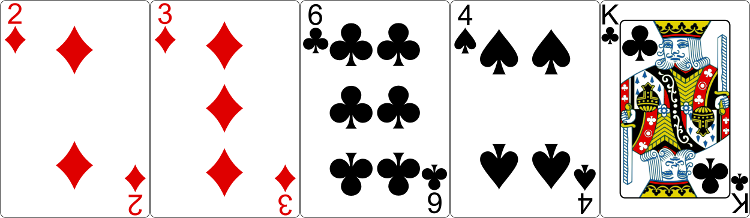
\includegraphics[width=\textwidth]{../img/w05-hands/none.png}
 \end{minipage}
 \begin{minipage}[c]{0.3\textwidth}
  \caption{Högt kort - inget mönster finns}
 \end{minipage}
\end{figure}

\subsection{Frivilliga extrauppgifter}

\Task Implementera metoden \code{tally} i klassen \code{Hand} så att simuleringen även kan registrera kortkombinationerna fyrtal, kåk, triss, tvåpar och par. Kör sedan \code{PokerProbability} igen.
